\begin{frame}{General framework for experiments}
	\begin{algorithm}[H]
		\small
		\begin{algorithmic}
			\Require{Sparse matrix $A$}
			\Ensure{Partitioning for the matrix $A$}
			\State Partition $A$ with Mondriaan using the medium-grain method
			\For{$i=1,\dots,iter_{max}$}
			\State Use any of the heuristics described previously to compute $A_r$ and $A_c$
			\State Construct $B$ from $A_r$ and $A_c$
			\State Partition $B$ with Mondriaan using the row-net model
			\State Re-construct $A$ with the new partitioning
			\EndFor
		\end{algorithmic}
	\end{algorithm}

	Unique framework for both partition-oblivious and partition-aware types of heuristics.

\end{frame}

\begin{frame}{Implementation}

	All of the heuristics have been implemented following these steps:

\begin{enumerate}\itemsep=0.3cm
		\item MATLAB prototyping
		\item Core C implementation (MATLAB compatibility through MEX files)
		\item Full C implementation
	\end{enumerate}

	The Hopcroft-Karp algorithm for the maximum independent set computation was implemented in the Python programming language.

\end{frame}

\begin{frame}{Implementation}

	Randomness involved during the computation of $A_r$ and $A_c$ and during the actual partitioning. To obtain meaningful results:

	\begin{itemize}
		\item 20 independent initial partitionings
		\item for each, 5 independent runs of the heuristic and subsequent partitioning ($iter_{max} = 1$)
	\end{itemize}

	18 matrices used for tests: 
	\begin{itemize}
		\item rectangular vs. square
		\item $10^{th}$ Dimacs Implementation Challenge
	\end{itemize}
\end{frame}

\begin{frame}{Preliminary selection}
	Wide selections of heuristics, preliminary selection is necessary.

	5 matrices used: 

	\begin{itemize}
		\item \texttt{dfl001};
		\item \texttt{tbdlinux};
		\item \texttt{nug30};
		\item \texttt{rgg\_n\_2\_18\_s0};
		\item  \texttt{bcsstk30}. 
	\end{itemize}

\end{frame}

\begin{frame}{Preliminary selection}

	Partition-oblivious heuristics (17 different algorithms):

	\begin{itemize}
		\item In general, results are much worse than medium-grain method.
		\item Mixing rows and columns in partial assignment is a bad idea
		\item Individual assignment of nonzero (\texttt{po\_localview}) is the best strategy (7\% worse than medium-grain)
		\item Maximum independent set computation (\texttt{po\_is}) yields interesting results (16\% lower communication volume in one matrix, but in general 12\% worse than medium-grain)
	\end{itemize}

	2 heuristics selected for deeper investigation.

\end{frame}

\begin{frame}{Preliminary selection}

	Partition-aware heuristics (21 different algorithms):

	\begin{itemize}
		\item Results closer to medium-grain efficiency
		\item SBD and SBD2 forms are not worthwile, nor individual assignment of nonzeros
		\item Refinement in sorting does not yield a substantial difference
		\item Unsorted concatenation of rows and columns (\texttt{pa\_row} and \texttt{pa\_col}) produces good results with rectangular matrices: they can be combined into a \texttt{po\_localbest} heuristic (which tries both and picks the best)
		\item Maximum independent set strategies (\texttt{pa\_is\_1} and \texttt{pa\_is\_3}) are very close to medium-grain, even better in a few matrices
	\end{itemize}

	5 heuristics selected for deeper investigation.

\end{frame}

\begin{frame}{Number of iterations}
	\begin{textblock}{170}(15,40)
		We are developing a fully iterative scheme: how many iterations do we have to execute?

		We run the 5 partition-aware selected heuristics for 10 consecutive iterations for each matrix

	\end{textblock}

	\only<1-5>{
		\vspace{1.5cm}
		\begin{figure}[h]
			\centering
			\only<1>{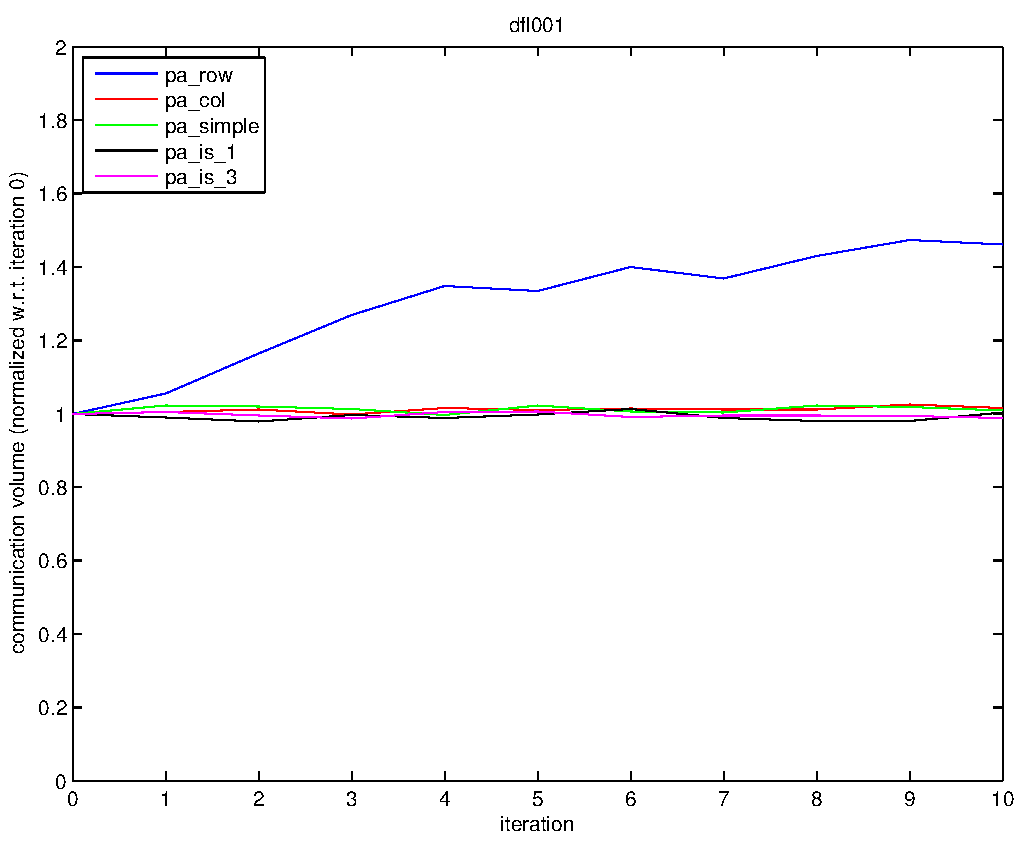
\includegraphics[scale=0.4]{../img/iter_dfl.pdf}}
			\only<2>{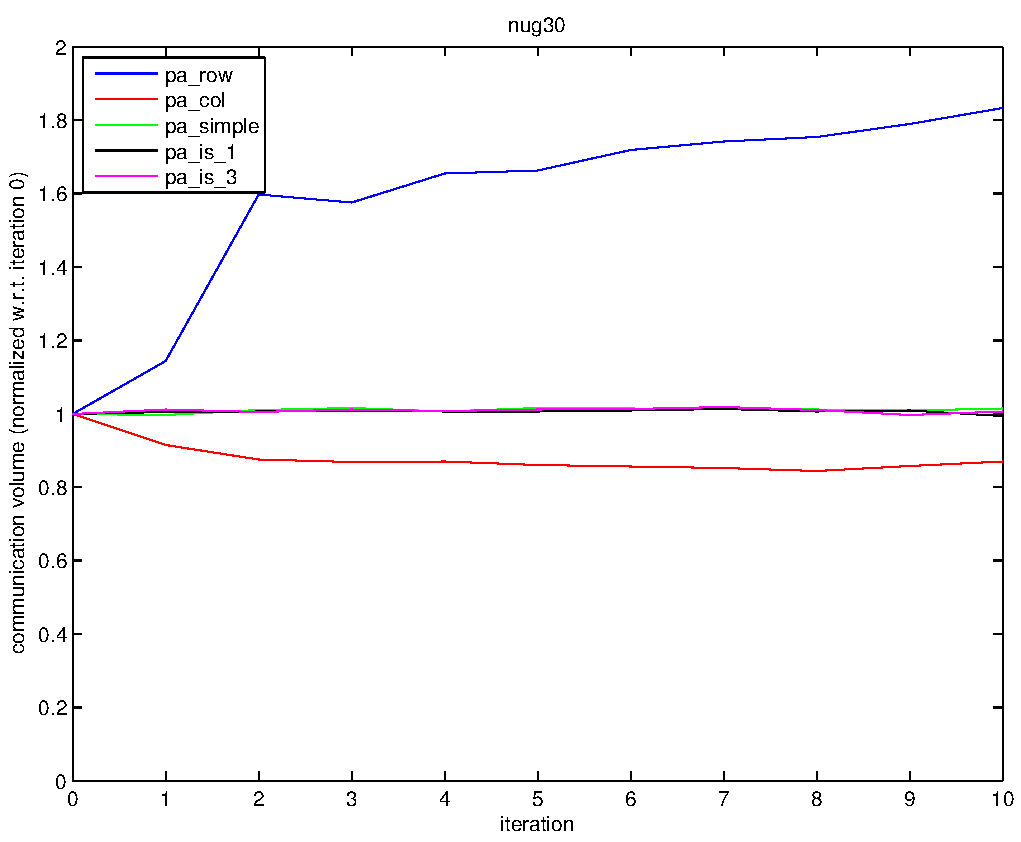
\includegraphics[scale=0.4]{../img/iter_nug30.pdf}}
			\only<3>{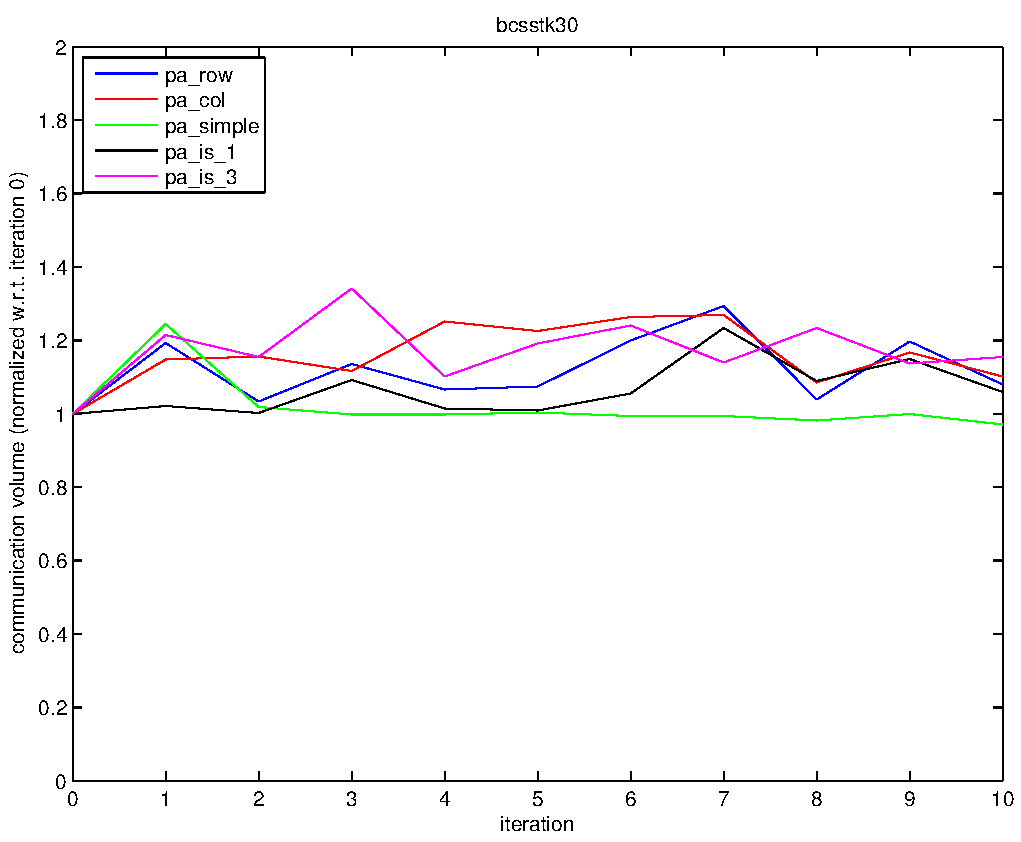
\includegraphics[scale=0.4]{../img/iter_bcs.pdf}}
			\only<4>{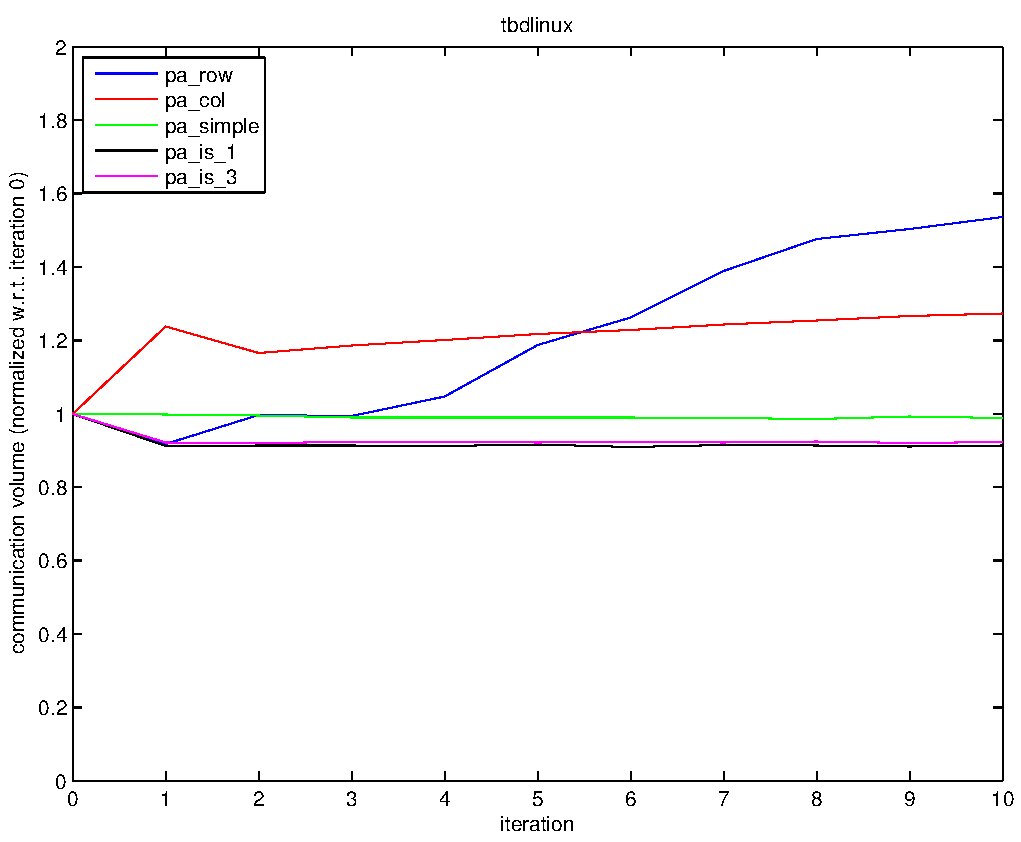
\includegraphics[scale=0.4]{../img/iter_tbdlinux.pdf}}
			\only<5>{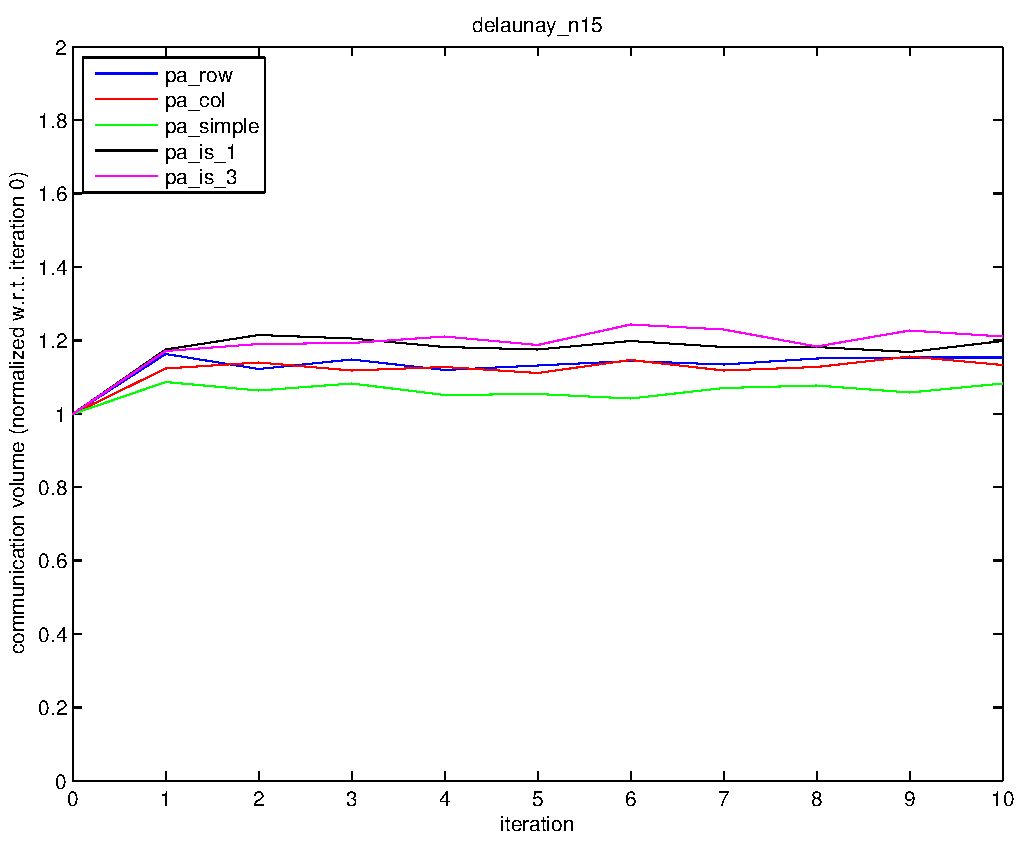
\includegraphics[scale=0.4]{../img/iter_delaunay.pdf}}
		\end{figure}
	}
	\only<6>{
	\begin{itemize}\itemsep=0.4cm
			\item Usually 1 iteration is enough to show improvements, if any.
			\item More iterations can worsen the communication volume.
		\end{itemize}
	}
\end{frame}

\begin{frame}{Analysis of the performance of the best heuristics}

	Partition-oblivious heuristics:

\begin{itemize}\itemsep=0.4cm
		\item No devised heuristic was able to improve medium-grain
		\item The preliminary results confirmed:

		\begin{itemize}\itemsep=0.3cm
				\item Individual assignment of nonzeros 7\% worse than medium-grain
				\item Computing the maximum independent set 22\% worse than medium-grain
			\end{itemize}
	\end{itemize}
\end{frame}

\begin{frame}{Analysis of the performance of the best heuristics}
	Partition-aware heuristics:

	\begin{itemize}
		\item Concatenation interesting strategy:
			\begin{itemize}
				\item \texttt{pa\_row} and \texttt{pa\_col} 8\% worse than medium-grain
				\item \texttt{localbest} method takes best of both: only 4\% worse than medium-grain 
			\end{itemize}
		\item Similar good results for the other strategies (between 4\% and 8\% higher communication volume than medium-grain)
		\item No algorithm was able to beat medium-grain
		\item Considering only rectangular matrices, our methods work better: they improve medium-grain, even if only by little (1-2\%)
	\end{itemize}
\end{frame}

\begin{frame}{Iterative refinement}
	\vspace{-0.2cm}

	Is there something we can do to improve the results?
	
	\vspace{0.2cm}

	Medium-grain employs a procedure of \textbf{iterative refinement}:

	\begin{enumerate}
		\item $A$ is partitioned into two sets ($A_0$ and $A_1$)
		\item we create again the matrix $B$ of the medium-grain method (example: $A_r = A_0$ and $A_c = A_1$)
		\item we retain communication volume: the first $n$ columns of $B$ are assigned to a single processor, and similarly for the other $m$
		\item we create the hypergraph from this $B$ and a single run of Kernighan-Lin is performed
		\item we repeat steps 1-4 until no improvement is found, then we swap the roles of $A_0$ and $A_1$ for the creation of $A_r$ and $A_c$
		\item we repeat step 5 until no other improvement is found
	\end{enumerate}

\end{frame}

\begin{frame}{Iterative refinement}
	Kernighan-Lin method is \textbf{monotonically non-increasing}: during iterative refinement, the communication volume is either lowered or remains at the same value.

Example of the construction of $B$:
\begin{figure}[h]
	\begin{tikzpicture}[scale=0.2]%,font=\large]
	\only<1->{	
		\foreach \x / \y in {1/1,1/3,2/2,4/5,4/4,3/11,4/9,6/7,1/10,2/7} { \fill[myred] ({\y-1},{-\x+1}) rectangle +(1,-1);}
		\foreach \x / \y in {1/2,2/3,3/6,3/9,6/6,5/1,5/12,6/10,2/11,2/8} { \fill[myblue] ({\y-1},{-\x+1}) rectangle +(1,-1);}
		\draw[thick] (0,-6) rectangle (12,0);
		\node at (6,-7) {$A$};
	}
		\visible<2->{
		\foreach \x / \y in {1/1,1/3,2/2,4/5,4/4,3/11,4/9,6/7,1/10,2/7}{ \fill[purple!90,opacity=.8] ({18+\y-1},{-6-\x+1}) rectangle +(1,-1);}
		\node at (24,-13) {$A_c$};
		\draw[thick] (18,{-6-6}) rectangle ({18+12},-6);

		\foreach \x / \y in  {1/2,2/3,3/6,3/9,6/6,5/1,5/12,6/10,2/11,2/8} { \fill[yellow!60!cyan,opacity=.9] ({18+\y-1},{6-\x+1}) rectangle +(1,-1);}
		\node at (24,-1) {$A_r$};
		\draw[thick] (18,{-6+6}) rectangle ({18+12},6);
		\draw[line width=1.3pt,>=latex,->] (13,-3) -- (17,-9);
		\draw[line width=1.3pt,>=latex,->] (13,-3) -- (17,3);
	}
\visible<3->{
	\only<-3>{
	\foreach \x / \y in {1/1,1/3,2/2,4/5,4/4,3/11,4/9,6/7,1/10,2/7}{ \fill[purple!90,opacity=.8] ({36+\y-1},{-6-\x+1}) rectangle +(1,-1);}
	\foreach \x / \y in  {1/2,2/3,3/6,3/9,6/6,5/1,5/12,6/10,2/11,2/8} { \fill[yellow!60!cyan,opacity=.9] ({48+\x-1},{6-\y+1}) rectangle +(1,-1);}
	\draw[line width=1.3pt,>=latex,->] (31,-9) -- (35,-4);
		\draw[line width=1.3pt,>=latex,->] (31,3) -- (35,-2);


		\foreach \x in {1,2,3,9,10,11} { \fill[gray!10!black,opacity=.9] ({36+\x-1},{6-\x+1}) rectangle +(1,-1);}
		\foreach \x in {1,2,3,6} { \fill[gray!10!black,opacity=.9] ({48+\x-1},{-6-\x+1}) rectangle +(1,-1);}

		\draw[thick] (36,-12) rectangle (54,6);
		\draw[ultra thick] (48,-12) -- (48,6);
		\draw[ultra thick] (36,-6) -- (54,-6);

		\node at (45,-13) {$B$};
	}\only<4->{
	\foreach \x / \y in {1/1,1/3,2/2,4/5,4/4,3/11,4/9,6/7,1/10,2/7}{ \fill[myred] ({36+\y-1},{-6-\x+1}) rectangle +(1,-1);}
	\foreach \x / \y in  {1/2,2/3,3/6,3/9,6/6,5/1,5/12,6/10,2/11,2/8} { \fill[myblue] ({48+\x-1},{6-\y+1}) rectangle +(1,-1);}
	\draw[line width=1.3pt,>=latex,->] (31,-9) -- (35,-4);
		\draw[line width=1.3pt,>=latex,->] (31,3) -- (35,-2);


		\foreach \x in {1,2,3,9,10,11} { \fill[myred] ({36+\x-1},{6-\x+1}) rectangle +(1,-1);}
		\foreach \x in {1,2,3,6} { \fill[myblue] ({48+\x-1},{-6-\x+1}) rectangle +(1,-1);}

		\draw[thick] (36,-12) rectangle (54,6);
		\draw[ultra thick] (48,-12) -- (48,6);
		\draw[ultra thick] (36,-6) -- (54,-6);

		\node at (45,-13) {$B$};
	}
	}
		
	\end{tikzpicture}
\end{figure}
\end{frame}

\begin{frame}{Iterative refinement}
	With iterative refinements, results are in general better:

	\begin{itemize}
		\item partition-oblivious algorithms:
			\begin{itemize}
				\item \texttt{po\_localview} still 7\% worse than medium-grain
				\item \texttt{po\_is} now 6\% worse than medium-grain (down from 22\%)
			\end{itemize}
		\item partition-aware algorithms:
			\begin{itemize}
				\item \texttt{pa\_row} and \texttt{pa\_col} now 2\% and 1\% worse than medium-grain (down from 8\%)
				\item \texttt{localbest} now 1\% \textbf{better} than medium-grain (down from 4\% worse)
				\item \texttt{pa\_simple} now 2\% worse than medium-grain (down from 4\%)
				\item \texttt{pa\_is\_1} and \texttt{pa\_is\_3} now 1\% worse than medium-grain (down from 5\% and 8\%)
			\end{itemize}
	\end{itemize}

	Now, with rectangular matrices, computing the independent set produces an average communication volume 4\% lower than medium-grain.

\end{frame}
